\chapter{Photon Orbits, Rindler Space, and the Schwarzschild Interior}

A Newtonian point mass and a Schwarzschild black hole begin with the same
idealization: all the gravitating mass is concentrated at the center.  Their
centers nevertheless have very different meanings.  In Newtonian mechanics a
particle with even a little angular momentum misses the center.  In a black
hole, once the particle has crossed the horizon, the singularity cannot be
missed.  Understanding that difference will take us through circular orbits,
the photon sphere, and finally a new set of coordinates near the horizon.

\section{A Center That Cannot Be Missed}

Real Newtonian matter never becomes a mathematical point.  Pressure, material
strength, and other forces resist compression.  Even if we nevertheless use a
point mass as an idealization, a falling particle rarely strikes it.  An
exactly radial trajectory can reach \(r=0\), but the slightest transverse
velocity supplies angular momentum.  The centrifugal barrier then turns the
particle around the center.

General relativity changes the conclusion.  A sufficiently compact body can
form a black hole, and the black-hole interior defeats the Newtonian escape by
going around the center.  The reason is deeper than a stronger force: inside
the horizon, decreasing \(r\) is a future direction.  We shall arrive at that
statement gradually rather than assume it.

\begin{classroomqa}
\audiencequestion{Is the Newtonian difficulty of hitting the center merely a
consequence of treating both objects as points?}
\lecturerresponse{The point idealization is part of the comparison, but it is
not the whole distinction.  In Newtonian mechanics any nonzero angular
momentum lets the orbit pass around the point.  In the relativistic interior,
the singularity lies to the future of every infalling time-like trajectory;
angular motion cannot provide an escape.
\lecturetimestamp{00:04:52--00:05:13}}
\end{classroomqa}

\section{Horizon and Singularity}

We take the Schwarzschild geometry as given for now:
\begin{equation}
d\tau^{2}
=
\left(1-\frac{2MG}{r}\right)dt^{2}
-
\frac{dr^{2}}{1-\frac{2MG}{r}}
-
r^{2}d\Omega^{2}.
\label{eq:l6-schwarzschild}
\end{equation}
The field equations that select this metric will come later.  Our immediate
task is to learn what the metric says.

One may write the metric on the unit sphere as
\begin{equation}
d\Omega^{2}
=d\vartheta^{2}+\cos^{2}\vartheta\,d\phi^{2}
\label{eq:l6-angular-metric}
\end{equation}
when \(\vartheta\) is latitude measured from the equatorial plane.  With the
more usual polar angle measured from the axis, the cosine becomes a sine.
Spherical symmetry lets every orbit be placed in one fixed plane, so only one
angular coordinate will survive in the calculation below.

\begin{figure}[htbp]
\centering

\includegraphics[width=0.88\textwidth]{lecture_06_figure_01.png}
\caption{The Schwarzschild metric and the cylindrical spacetime picture of
the surface \(r=2MG\).  The central line is \(r=0\); the red cylinder is the
horizon in Schwarzschild coordinates.}
\lectureframe{00:09:45}
\end{figure}

Far from the source, \(2MG/r\) is small and
Eq.~\eqref{eq:l6-schwarzschild} approaches the Minkowski metric in spherical
coordinates.  Two radii stand out:
\begin{equation}
r=2MG,
\qquad
r=0.
\end{equation}
They must not be confused.  At \(r=2MG\), the coefficient of \(dt^{2}\)
vanishes and that of \(dr^{2}\) diverges.  The Schwarzschild coordinate system
has become singular.  The curvature itself remains finite there.  At \(r=0\),
by contrast, curvature invariants diverge.  The tidal field stretches an
extended body radially and squeezes it transversely without bound.  That is a
physical singularity, not a defect in the coordinates.

\subsection{Two Ways of Timing a Fall}

For a stationary clock outside the horizon,
\begin{equation}
d\tau
=
\sqrt{1-\frac{2MG}{r}}\,dt.
\label{eq:l6-static-clock}
\end{equation}
At large \(r\), \(d\tau\simeq dt\).  Near the horizon, the proper time of a
clock held at fixed \(r\) advances very slowly relative to the Schwarzschild
time kept far away.

The same coordinates describe radial infall as taking an infinite value of
\(t\) to reach \(r=2MG\).  The infaller's own elapsed proper time is finite.
There is no conflict between those statements.  A clock carried by the
infaller measures the proper time along its worldline.  It may be a mechanical
clock, a light clock made from mirrors at the ends of a meter stick, a
heartbeat, or the succession of physical processes in a brain.  None of these
measures the distant coordinate \(t\).  The distinction between the two clocks
will become visible in the near-horizon diagram.

\section{Circular Motion from the Proper-Time Action}

Before returning to infall, let us solve a different problem: under what
conditions can a massive particle or a photon circle the black hole?  The
calculation begins with the same action principle used for any freely moving
relativistic particle,
\begin{equation}
S=-m\int d\tau.
\label{eq:l6-particle-action}
\end{equation}
Light is bent by the Earth, but the terrestrial field is nowhere near strong
enough to close a light ray into an orbit.  The Earth's Schwarzschild radius
is only of order a centimeter.  One would have to compress the whole Earth to
roughly that scale, about the size of a small nut, before the strong-field
question became relevant.

Set \(c=1\), restrict the motion to an equatorial plane, and define
\begin{equation}
F(r)=1-\frac{2MG}{r},
\qquad
G(r)=\frac{1}{F(r)}.
\label{eq:l6-fg}
\end{equation}
Using the coordinate time \(t\) as the parameter gives
\begin{equation}
d\tau
=dt\sqrt{F-G\dot r^{\,2}-r^{2}\dot\theta^{\,2}},
\end{equation}
and therefore
\begin{equation}
\mathcal L
=
-m\sqrt{F-G\dot r^{\,2}-r^{2}\dot\theta^{\,2}}.
\label{eq:l6-lagrangian}
\end{equation}
The factor \(m\) gives the action its usual dimensions of energy times time.

\begin{figure}[htbp]
\centering

\includegraphics[width=0.76\textwidth]{lecture_06_figure_02.png}
\caption{The square-root particle Lagrangian being assembled on the board.
The complete expression is given in Eq.~\eqref{eq:l6-lagrangian}.}
\lectureframe{00:31:53}
\end{figure}

For any generalized coordinate \(q\),
\begin{equation}
p_q=\frac{\partial\mathcal L}{\partial\dot q}.
\end{equation}
It is useful to reserve \(\mathcal L\) for the Lagrangian and \(L\) for the
angular momentum.  With
\begin{equation}
\Delta=F-G\dot r^{\,2}-r^{2}\dot\theta^{\,2},
\end{equation}
the two momenta are
\begin{align}
L=p_\theta
&=\frac{mr^{2}\dot\theta}{\sqrt{\Delta}},
\label{eq:l6-angular-momentum}\\
p_r
&=\frac{mG\dot r}{\sqrt{\Delta}}.
\label{eq:l6-radial-momentum}
\end{align}
The radial momentum is not conserved because the radial coordinate appears in
the Lagrangian.  The angle \(\theta\) does not appear, so \(L\) is conserved.

There is also no explicit \(t\) in \(\mathcal L\).  The Hamiltonian is
therefore conserved:
\begin{align}
E=H
&=p_r\dot r+L\dot\theta-\mathcal L \\
&=\frac{mG\dot r^{\,2}}{\sqrt{\Delta}}
  +\frac{mr^{2}\dot\theta^{\,2}}{\sqrt{\Delta}}
  +m\sqrt{\Delta} \\
&=\frac{mF}{\sqrt{\Delta}}.
\label{eq:l6-energy-general}
\end{align}
This is a characteristic rhythm of mechanics.  A principle gives the action;
a calculation gives the momenta; symmetry then turns the calculation back
into the principles of energy and angular-momentum conservation.  One could
immediately solve all the Euler--Lagrange equations, but the constants supplied
by rotational and time-translation symmetry eliminate much of that work.

\subsection{The Circular-Orbit Energy}

For a circular orbit,
\begin{equation}
\dot r=0.
\end{equation}
Introduce the angular momentum per unit mass,
\begin{equation}
\lambda=\frac{L}{m}.
\end{equation}
Equations~\eqref{eq:l6-angular-momentum} and
\eqref{eq:l6-energy-general} become
\begin{align}
\lambda
&=\frac{r^{2}\dot\theta}
{\sqrt{F-r^{2}\dot\theta^{\,2}}},
\label{eq:l6-lambda-circular}\\
E
&=\frac{mF}{\sqrt{F-r^{2}\dot\theta^{\,2}}}.
\label{eq:l6-energy-circular-first}
\end{align}

\begin{figure}[htbp]
\centering

\includegraphics[width=0.82\textwidth]{lecture_06_figure_04.png}
\caption{The reduced angular momentum and energy for circular Schwarzschild
motion.  The angular-momentum equation is used first to eliminate
\(\dot\theta\) from the energy.}
\lectureframe{00:39:14}
\end{figure}

Squaring Eq.~\eqref{eq:l6-lambda-circular} and solving for the angular
velocity gives
\begin{equation}
\dot\theta^{\,2}
=
\frac{\lambda^{2}F}
{r^{2}\left(r^{2}+\lambda^{2}\right)}.
\label{eq:l6-angular-speed}
\end{equation}
Substitution into Eq.~\eqref{eq:l6-energy-circular-first} leaves an energy that
depends only on the proposed radius and the fixed angular momentum:
\begin{equation}
E(r,\lambda)
=m\sqrt{F(r)}\,\frac{\sqrt{r^{2}+\lambda^{2}}}{r}.
\label{eq:l6-circular-energy}
\end{equation}

The class pauses over a Newtonian comparison.  In an ordinary circular orbit,
the angular frequency and the tangential speed decrease as the radius grows,
but the angular momentum includes a factor of radius.  One should therefore
not infer the behavior of \(L\) from the angular speed alone.  The relativistic
formula keeps those factors explicit.

\section{The Circular Orbit of Light}

A photon has energy and momentum even though its rest mass vanishes.  The
massless limit of Eq.~\eqref{eq:l6-circular-energy} must consequently be taken
with care.  If \(m\) went to zero at fixed \(\lambda\), then
\(L=m\lambda\) would also vanish.  Instead take
\begin{equation}
m\longrightarrow0,
\qquad
\lambda\longrightarrow\infty,
\qquad
L=m\lambda\ \text{fixed}.
\label{eq:l6-massless-limit}
\end{equation}
The \(\lambda^{2}\) term then dominates, and the photon energy becomes
\begin{equation}
E_\gamma(r;L)
=L\,\frac{\sqrt{1-\frac{2MG}{r}}}{r}.
\label{eq:l6-photon-energy}
\end{equation}
The factor \(L\) multiplies the entire radial function.  It affects the energy
scale but not the radius of a circular orbit.

\begin{figure}[htbp]
\centering

\includegraphics[width=0.88\textwidth]{lecture_06_figure_05.png}
\caption{The radial factor in the photon energy.  It vanishes at the horizon,
falls toward zero at large radius, and has one maximum between them.}
\lectureframe{00:50:50}
\end{figure}

At fixed \(L\), radial equilibrium requires a stationary point:
\begin{equation}
\frac{d}{dr}
\left[
\frac{\sqrt{1-\frac{2MG}{r}}}{r}
\right]=0.
\end{equation}
Differentiating,
\begin{equation}
-\frac{\sqrt{1-\frac{2MG}{r}}}{r^{2}}
+
\frac{MG}
{r^{3}\sqrt{1-\frac{2MG}{r}}}
=0,
\end{equation}
and hence
\begin{equation}
r=3MG.
\label{eq:l6-photon-sphere}
\end{equation}
This radius is one and a half times the Schwarzschild radius.  It is usually
called the photon sphere.

The stationary point is a maximum, so the circular photon orbit is unstable.
A photon placed exactly at \(3MG\) remains there.  An arbitrarily small radial
displacement eventually sends it away from the maximum.  Just outside the
photon sphere, a ray can sweep through a very large angle, perhaps winding
around the hole many times, before escaping.  Just inside it, a nearly
tangential ray can wind several times and then fall through the horizon.

\begin{figure}[htbp]
\centering
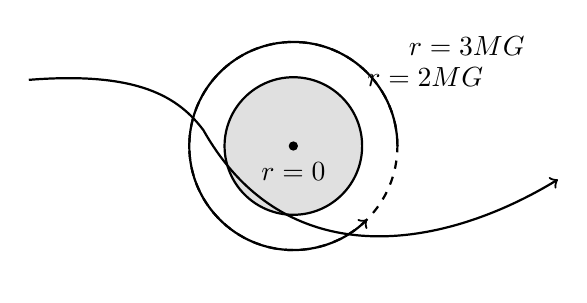
\begin{tikzpicture}[scale=1.12]
\fill[black!12] (0,0) circle (0.78);
\draw[thick] (0,0) circle (0.78);
\draw[dashed,thick] (0,0) circle (1.18);
\fill (0,0) circle (1.5pt);
\draw[->,thick] (1.18,0) arc (0:315:1.18);
\draw[->,thick] (-3.0,0.75)
  .. controls (-1.75,0.85) and (-1.30,0.55) .. (-1.02,0.18)
  .. controls (-0.10,-1.45) and (1.65,-1.20) .. (3.0,-0.38);
\node[right] at (0.73,0.78) {\(r=2MG\)};
\node[right] at (1.20,1.13) {\(r=3MG\)};
\node[below] at (0,-0.08) {\(r=0\)};
\end{tikzpicture}
\caption{The horizon, the photon sphere, and a strongly deflected ray.  Rays
arbitrarily close to the unstable circular orbit can accumulate arbitrarily
large deflection before escaping or falling inward.}
\end{figure}

\begin{classroomqa}
\audiencequestion{Why hold angular momentum fixed, and how is it related to a
photon's frequency and incoming trajectory?}
\lecturerresponse{Every ray carries a conserved angular momentum about the
black hole.  Its frequency fixes the magnitude of its linear momentum, while
its offset from the center helps determine \(L\).  Away from a circular orbit,
radius and angular momentum may be chosen independently.  Requiring a
circular photon orbit links the motion to the unique radius \(3MG\), and the
factorization in Eq.~\eqref{eq:l6-photon-energy} shows that this radius is
independent of the magnitude of \(L\).
\lecturetimestamp{00:54:43--00:57:02}}
\end{classroomqa}

\begin{classroomqa}
\audiencequestion{Why does the maximum of the energy locate an orbit?}
\lecturerresponse{After the angular motion has been eliminated at fixed
\(L\), the remaining function plays the role of an effective radial energy.
A stationary point supplies radial equilibrium.  A minimum would be stable;
this point is a maximum and therefore gives an unstable circular orbit.  There
is no contradiction in calling it an equilibrium and unstable at the same
time.
\lecturetimestamp{00:57:51--00:58:54}}
\end{classroomqa}

A massive particle can have time-like circular orbits outside \(3MG\), though
those nearest the photon sphere are unstable.  A massless particle has only
the circular orbit at \(3MG\).  Inside the photon sphere, a tangentially moving
photon falls inward; an object moving more slowly has no better chance of
maintaining such an orbit.  This statement concerns angular motion.  Outside
the horizon, a sufficiently outward-directed ray can still escape even when
its starting radius is below \(3MG\).

\section{What a Black Hole Does to an Image}

The photon sphere explains why a black hole is not merely a dark disk pasted
over an otherwise unchanged sky.  Light from a background object can reach an
observer along several paths.  One ray may pass on one side of the hole,
another on the other side, and still others may circle the hole one or more
times.  The result can contain displaced images, duplicated images, rings, and
an infinite sequence of ever finer, ever fainter images associated with
additional windings.  The exact picture is complicated, but its origin is
already contained in the unstable orbit.

When source, lens, and observer are sufficiently aligned, the image can form
an Einstein ring.  Gravitational-lensing rings are observed in nature.  The
full black-hole image requires integrating the null geodesics for many initial
directions, a calculation well suited to a computer.

\begin{classroomqa}
\audiencequestion{Does this optical boundary refer to the photon sphere or to
the horizon?}
\lecturerresponse{They play different roles.  The horizon at \(2MG\) is the
causal boundary: no future-directed signal escapes from inside it.  The photon
sphere at \(3MG\) controls tangential motion and strong lensing.  Between the
two radii, an outward radial ray can escape, while a tangential ray falls in.
Intermediate directions may loop before escaping or being captured.
\lecturetimestamp{01:02:47--01:03:40}}
\end{classroomqa}

\begin{classroomqa}
\audiencequestion{Can a general light path be calculated rather than merely
sketched?}
\lecturerresponse{Yes.  Insert the null condition into the geodesic or
Euler--Lagrange equations and integrate with the chosen initial data.  The
equations are not conceptually new, but the ray tracing is algebraically
messy, which is why numerical calculation is the practical method for an
image.
\lecturetimestamp{01:03:48--01:04:27}}
\end{classroomqa}

\begin{classroomqa}
\audiencequestion{Would applying the Euler--Lagrange equations directly have
made the circular-orbit calculation harder?}
\lecturerresponse{It would give the same result.  The action is the proper
starting point in either method, but the cyclic coordinates expose conserved
energy and angular momentum.  Using those constants first is the shorter
route to the circular-orbit condition.
\lecturetimestamp{01:04:33--01:05:49}}
\end{classroomqa}

\section{The Near-Horizon Metric Is Rindler Space}

We now return to the horizon.  The Schwarzschild coefficients appear to blow
up or vanish there, and on crossing the horizon their signs exchange.  Yet an
infalling observer encounters no divergent local curvature at that surface.
The equivalence principle tells us how both statements can be true.

Begin with two-dimensional Minkowski spacetime:
\begin{equation}
d\tau^{2}=dT^{2}-dX^{2}.
\end{equation}
In the right Rindler wedge define
\begin{equation}
X=\rho\cosh\omega,
\qquad
T=\rho\sinh\omega.
\label{eq:l6-rindler-map}
\end{equation}
Curves of constant \(\rho\) obey
\begin{equation}
X^{2}-T^{2}=\rho^{2},
\end{equation}
so they are hyperbolae, the worldlines of uniformly accelerated observers.
Substituting Eq.~\eqref{eq:l6-rindler-map} into the flat metric gives
\begin{equation}
d\tau^{2}
=\rho^{2}d\omega^{2}-d\rho^{2}.
\label{eq:l6-rindler-metric}
\end{equation}
Now set
\begin{equation}
\rho^{2}=4\xi,
\qquad
\omega=\frac{t}{2}.
\label{eq:l6-rindler-rescale}
\end{equation}
Since \(d\rho^{2}=d\xi^{2}/\xi\), Eq.~\eqref{eq:l6-rindler-metric}
becomes
\begin{equation}
d\tau^{2}
=\xi\,dt^{2}-\frac{d\xi^{2}}{\xi}.
\label{eq:l6-xi-metric}
\end{equation}

\begin{classroomqa}
\audiencequestion{Where have the angular or transverse coordinates gone?}
\lecturerresponse{They have only been suppressed.  We are examining the local
\(t\)-\(r\) plane that contains the horizon-crossing behavior.  The two
transverse directions remain regular and can be restored; they do not change
the coordinate singularity being analyzed.
\lecturetimestamp{01:16:27--01:16:47}}
\end{classroomqa}

To compare with Schwarzschild, choose units in which \(2MG=1\).  The radial
part of Eq.~\eqref{eq:l6-schwarzschild} is
\begin{equation}
d\tau^{2}
=
\frac{r-1}{r}\,dt^{2}
-
\frac{r}{r-1}\,dr^{2}.
\end{equation}
Very near \(r=1\), the small numerator \(r-1\) must be retained, while the
otherwise harmless factors of \(r\) may be replaced by one.  Thus
\begin{equation}
d\tau^{2}
\simeq
(r-1)\,dt^{2}
-
\frac{dr^{2}}{r-1}.
\end{equation}
With
\begin{equation}
\xi=r-1,
\end{equation}
this is exactly Eq.~\eqref{eq:l6-xi-metric}.  The near-horizon Schwarzschild
geometry is locally the Rindler description of flat spacetime.

\begin{classroomqa}
\audiencequestion{How can these be accelerated coordinates if the underlying
spacetime is flat?}
\lecturerresponse{Acceleration belongs to the observer, not necessarily to
curvature.  A worldline at fixed \(\rho\) is uniformly accelerated in
Minkowski spacetime.  Likewise, an observer held at fixed radius near a black
hole must be supported against free fall.  The equivalence principle makes
the local descriptions agree even though the complete Schwarzschild
spacetime is curved.
\lecturetimestamp{01:22:19--01:24:06}}
\end{classroomqa}

\section{Crossing the Rindler Horizon}

The right-wedge formulas cover only \(\xi>0\):
\begin{equation}
X=2\sqrt{\xi}\cosh\frac{t}{2},
\qquad
T=2\sqrt{\xi}\sinh\frac{t}{2}.
\label{eq:l6-rindler-outside}
\end{equation}
The surface \(\xi=0\) is the null line \(X=T\).  To continue into the future
wedge, let
\begin{equation}
\zeta=-\xi>0
\end{equation}
and interchange the hyperbolic roles:
\begin{equation}
T=2\sqrt{\zeta}\cosh\frac{t}{2},
\qquad
X=2\sqrt{\zeta}\sinh\frac{t}{2}.
\label{eq:l6-rindler-inside}
\end{equation}
The metric is still
\begin{equation}
d\tau^{2}
=\xi\,dt^{2}-\frac{d\xi^{2}}{\xi},
\end{equation}
but when \(\xi<0\), the coefficient of \(dt^{2}\) is negative and the
coefficient of \(d\xi^{2}\) is positive.  The coordinate \(\xi\), and hence
the Schwarzschild radial direction, has become time-like; \(t\) has become
space-like.

\begin{figure}[htbp]
\centering

\includegraphics[width=0.88\textwidth]{lecture_06_figure_06.png}
\caption{The Rindler wedges, their null boundaries, and the continuation from
\(\xi>0\) to \(\xi<0\).  The board also records
\(\rho^{2}=4\xi\) and \(\omega=t/2\).}
\lectureframe{01:29:40}
\end{figure}

\begin{classroomqa}
\audiencequestion{Do some curves in this coordinate drawing move faster than
light?}
\lecturerresponse{A coordinate grid line need not be the worldline of a
material object.  Its coordinate slope can look superluminal without
violating causality.  Physical light rays remain on the null lines, and
physical particles remain inside their local light cones.
\lecturetimestamp{01:28:44--01:29:08}}
\end{classroomqa}

Continuing farther into the Schwarzschild interior eventually brings us to
\(r=0\).  That boundary is space-like.  It is therefore better described as a
time than as a place: every future-directed time-like or null trajectory in
the black-hole interior reaches it.  One may go around a place.  One cannot go
around one's future.

\begin{classroomqa}
\audiencequestion{Could the diagram simply continue through \(r=0\) to
negative \(r\), and is \(r=0\) still the center?}
\lecturerresponse{The coordinate drawing may tempt us to extend a line, but
the classical Schwarzschild solution ends at the curvature singularity.
\(r=0\) may still be called the center, but it is a very unusual center: in
the interior it is a space-like future boundary.  There is no regular passage
through it to a negative-radius region.
\lecturetimestamp{01:32:16--01:34:06}}
\end{classroomqa}

\begin{classroomqa}
\audiencequestion{Are the diagonal axes in the Rindler diagram light-like,
and can an infaller enter at a finite value of the accelerated time?}
\lecturerresponse{Yes, the wedge boundaries are null lines.  A freely falling
worldline crosses such a line at an ordinary finite event and in finite
proper time.  The accelerated coordinate \(t\), or equivalently
\(\omega\), runs without bound along the exterior constant-\(\rho\)
description; it is that coordinate assignment, not the crossing event, that
becomes infinite.
\lecturetimestamp{01:34:26--01:35:03}}
\end{classroomqa}

\section{Alice Outside and Bob Falling}

Let Alice remain outside at fixed radius, supported against gravity, and let
Bob fall freely.  Near the horizon, Alice follows a Rindler-like hyperbola.
Her constant-\(t\) slices crowd ever closer to the null boundary.  Every event
on Bob's worldline that Alice labels with a finite \(t\) lies outside the
horizon, so she never assigns a finite Schwarzschild time to his crossing.

Bob carries a proper-time clock.  His trajectory cuts across the null line in
a finite interval of that clock.  Nothing locally divergent happens as he
crosses.  The horizon is globally decisive but locally ordinary.

\begin{figure}[htbp]
\centering
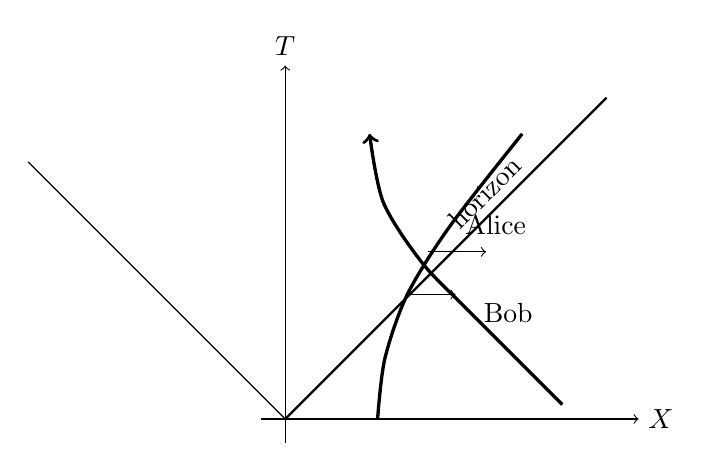
\begin{tikzpicture}[scale=1.02]
\draw[->] (-0.3,0) -- (4.4,0) node[right] {\(X\)};
\draw[->] (0,-0.3) -- (0,4.4) node[above] {\(T\)};
\draw[thick] (0,0) -- (4.0,4.0);
\draw[thin] (0,0) -- (-3.2,3.2);
\node[rotate=45,above] at (2.65,2.65) {horizon};
\draw[very thick]
  plot[smooth] coordinates {(1.15,0.0) (1.24,0.75) (1.52,1.55)
  (2.05,2.40) (2.95,3.55)};
\node[right] at (2.12,2.42) {Alice};
\draw[very thick,->]
  plot[smooth] coordinates {(3.45,0.18) (2.85,0.78) (2.25,1.38)
  (1.70,1.95) (1.22,2.70) (1.05,3.55)};
\node[right] at (2.35,1.32) {Bob};
\draw[->] (1.52,1.55) -- (2.12,1.55);
\draw[->] (1.78,2.08) -- (2.50,2.08);
\end{tikzpicture}
\caption{Alice's accelerated exterior worldline and Bob's freely falling
worldline.  Alice's coordinate slices approach the horizon; Bob crosses it in
finite proper time.}
\end{figure}

\begin{classroomqa}
\audiencequestion{What does Bob see when he looks back at Alice, and what
becomes of his clock after crossing?}
\lecturerresponse{Bob sees Alice receding with the acceleration required to
hold her outside, but he does not see a singular event at his crossing.
Alice may be supported at fixed radius; an orbit is a different possible
setup.  Bob's clock continues to measure his proper time \(\tau\) normally.
Inside, saying that the radial coordinate is time-like describes the causal
geometry; it does not literally turn his wristwatch into a meter stick.  His
worldline finally ends at \(r=0\).
\lecturetimestamp{01:39:51--01:44:45}}
\end{classroomqa}

The null line is now recognized as the horizon itself, not merely as one point
where a coordinate coefficient misbehaves.  Outside it, one family of radial
light rays moves outward.  Inside it, both future light-cone directions lead
toward smaller \(r\).  Every future-directed massive trajectory must remain
between those null directions and therefore reaches the singularity.

\section{Signals, Redshift, and a Forming Horizon}

Suppose collapsing matter emits a regular sequence of light pulses.  A distant
observer receives the later pulses at increasingly long intervals.  Their
frequencies shift from optical toward infrared, microwave, radio, and still
longer wavelengths.  In an idealized classical calculation the outside
observer can continue to associate ever later signals with matter approaching
the horizon, but the source rapidly becomes too red and too faint to detect in
practice.

\begin{classroomqa}
\audiencequestion{During collapse, does an outside observer see all the
matter simply freeze at the horizon?}
\lecturerresponse{In Schwarzschild time, the surface of the collapsing matter
approaches the horizon asymptotically and appears increasingly frozen.  What
is actually observed is encoded in light signals, and those signals become
more delayed, redshifted, and faint.  This coordinate account does not say
that the infalling matter experiences an infinite proper time.
\lecturetimestamp{01:47:06--01:48:11}}
\end{classroomqa}

\begin{classroomqa}
\audiencequestion{Could a sufficiently late observer recover the entire
history of the fall?}
\lecturerresponse{Only through signals that were emitted and manage to reach
the observer.  Successive pulses are increasingly separated and redshifted.
An ideal observer with unlimited sensitivity could follow the classical
signal to ever longer wavelengths; a practical observer sees the object fade
away.
\lecturetimestamp{01:48:13--01:52:00}}
\end{classroomqa}

\begin{classroomqa}
\audiencequestion{What precisely is meant by saying that the singularity is
a time rather than a place?}
\lecturerresponse{The \(r=0\) surface is space-like.  Once inside the
horizon, every future-directed time-like or null curve terminates there.  A
spatial location can be avoided by choosing another route; a future boundary
cannot be avoided while continuing along a future-directed worldline.
\lecturetimestamp{01:52:02--01:53:10}}
\end{classroomqa}

How, then, can a black hole form or increase its mass if the outside observer
never sees matter cross?  Consider a collapsing spherical shell.  The global
horizon does not wait as a pre-existing material surface at one fixed radius.
It begins at the center and grows outward, meeting the collapsing shell as the
black-hole region forms.  The external Schwarzschild description still makes
the shell approach the final horizon asymptotically.  The complete spacetime
picture, including how the horizon is located globally, is the subject of the
next lecture.

\begin{figure}[htbp]
\centering

\includegraphics[width=0.90\textwidth]{lecture_06_figure_07.png}
\caption{A collapsing shell and the horizon growing outward from the center
to meet it.  The drawing is a preview of the global collapse geometry
developed in the next lecture.}
\lectureframe{01:57:25}
\end{figure}

\begin{classroomqa}
\audiencequestion{If nothing crosses the horizon in the external coordinate
time, how can a black hole form or grow?}
\lecturerresponse{The premise mixes a coordinate statement with a global
one.  The collapsing matter reaches the relevant region in finite proper
time, while the event horizon is determined by the causal structure of the
whole spacetime.  In the shell picture it starts at the center and grows
outward to meet the shell.  The outside observer's delayed, redshifted view is
still consistent with that global horizon.
\lecturetimestamp{01:53:11--01:57:34}}
\end{classroomqa}

\section{Escape Directions Between the Two Spheres}

The horizon and photon sphere divide the ray problem into distinct cases.  At
a radius
\begin{equation}
2MG<r<3MG,
\end{equation}
a radially outgoing light ray can escape to infinity.  A tangential light ray
cannot; it falls inward.  Between those directions lies an escape cone.
Closer to the horizon, that cone narrows around the outward radial direction.
After the horizon is crossed, it closes completely.

\begin{classroomqa}
\audiencequestion{Can a light source between the horizon and photon sphere
send any signal outward?}
\lecturerresponse{Yes.  A sufficiently radial outward null ray escapes as
long as its emission event is outside \(2MG\).  The statement that angular
motion inside \(3MG\) falls inward does not forbid radial escape.  The outcome
depends on the emission direction, and the allowed outward cone narrows as
the source approaches the horizon.
\lecturetimestamp{01:57:34--01:59:48}}
\end{classroomqa}

\begin{classroomqa}
\audiencequestion{Can a ray arriving from outside cross inside the photon
sphere, turn around, and emerge again?}
\lecturerresponse{Not along a null geodesic of the type under discussion.  A
turning point would have zero radial velocity, so the ray would momentarily be
tangential at a radius below \(3MG\); there the angular trajectory falls
inward rather than turning back out.  A source already between the two
spheres can nevertheless emit a sufficiently radial outward ray before it
crosses the horizon.
\lecturetimestamp{01:59:49--02:01:27}}
\end{classroomqa}

The last question is intentionally less settled.  Imagine Alice and Bob both
held at the same radius outside the horizon.  Nearby observers can plainly
exchange signals.  If they are far apart around the sphere, the direct null
path and its limiting angular range require an explicit geodesic
calculation.  The class proposes an indirect route: send the message nearly
radially outward to a relay at a safer radius, carry it around there, and send
it back inward.  Another version lets an outward-thrown object or signal turn
around and return.  These routes show why failure of a tangential circular
orbit does not by itself forbid all communication between exterior
observers.

\begin{classroomqa}
\audiencequestion{Can two observers suspended at the same near-horizon radius
communicate around the black hole?}
\lecturerresponse{Locally, yes.  For widely separated or diametrically
opposite observers, the direct-path limit was not worked out in the lecture
and should not be promoted to a theorem.  The discussion first leaves that
angular-geodesic question open, then observes that an indirect signal can go
nearly radially outward, be relayed around at larger radius, and return.
Approaching the horizon makes the directly useful angular range increasingly
narrow, but outside the horizon an outward route remains available.
\lecturetimestamp{02:01:29--02:04:17}}
\end{classroomqa}

The next step is to replace these near-horizon sketches by the global geometry
of a collapsing body and to see precisely how an event horizon grows.
